\documentclass[tikz,border=10pt]{standalone}
\usetikzlibrary{arrows.meta, positioning, calc}
\usepackage{amsmath}
\usepackage{amssymb}

\begin{document}
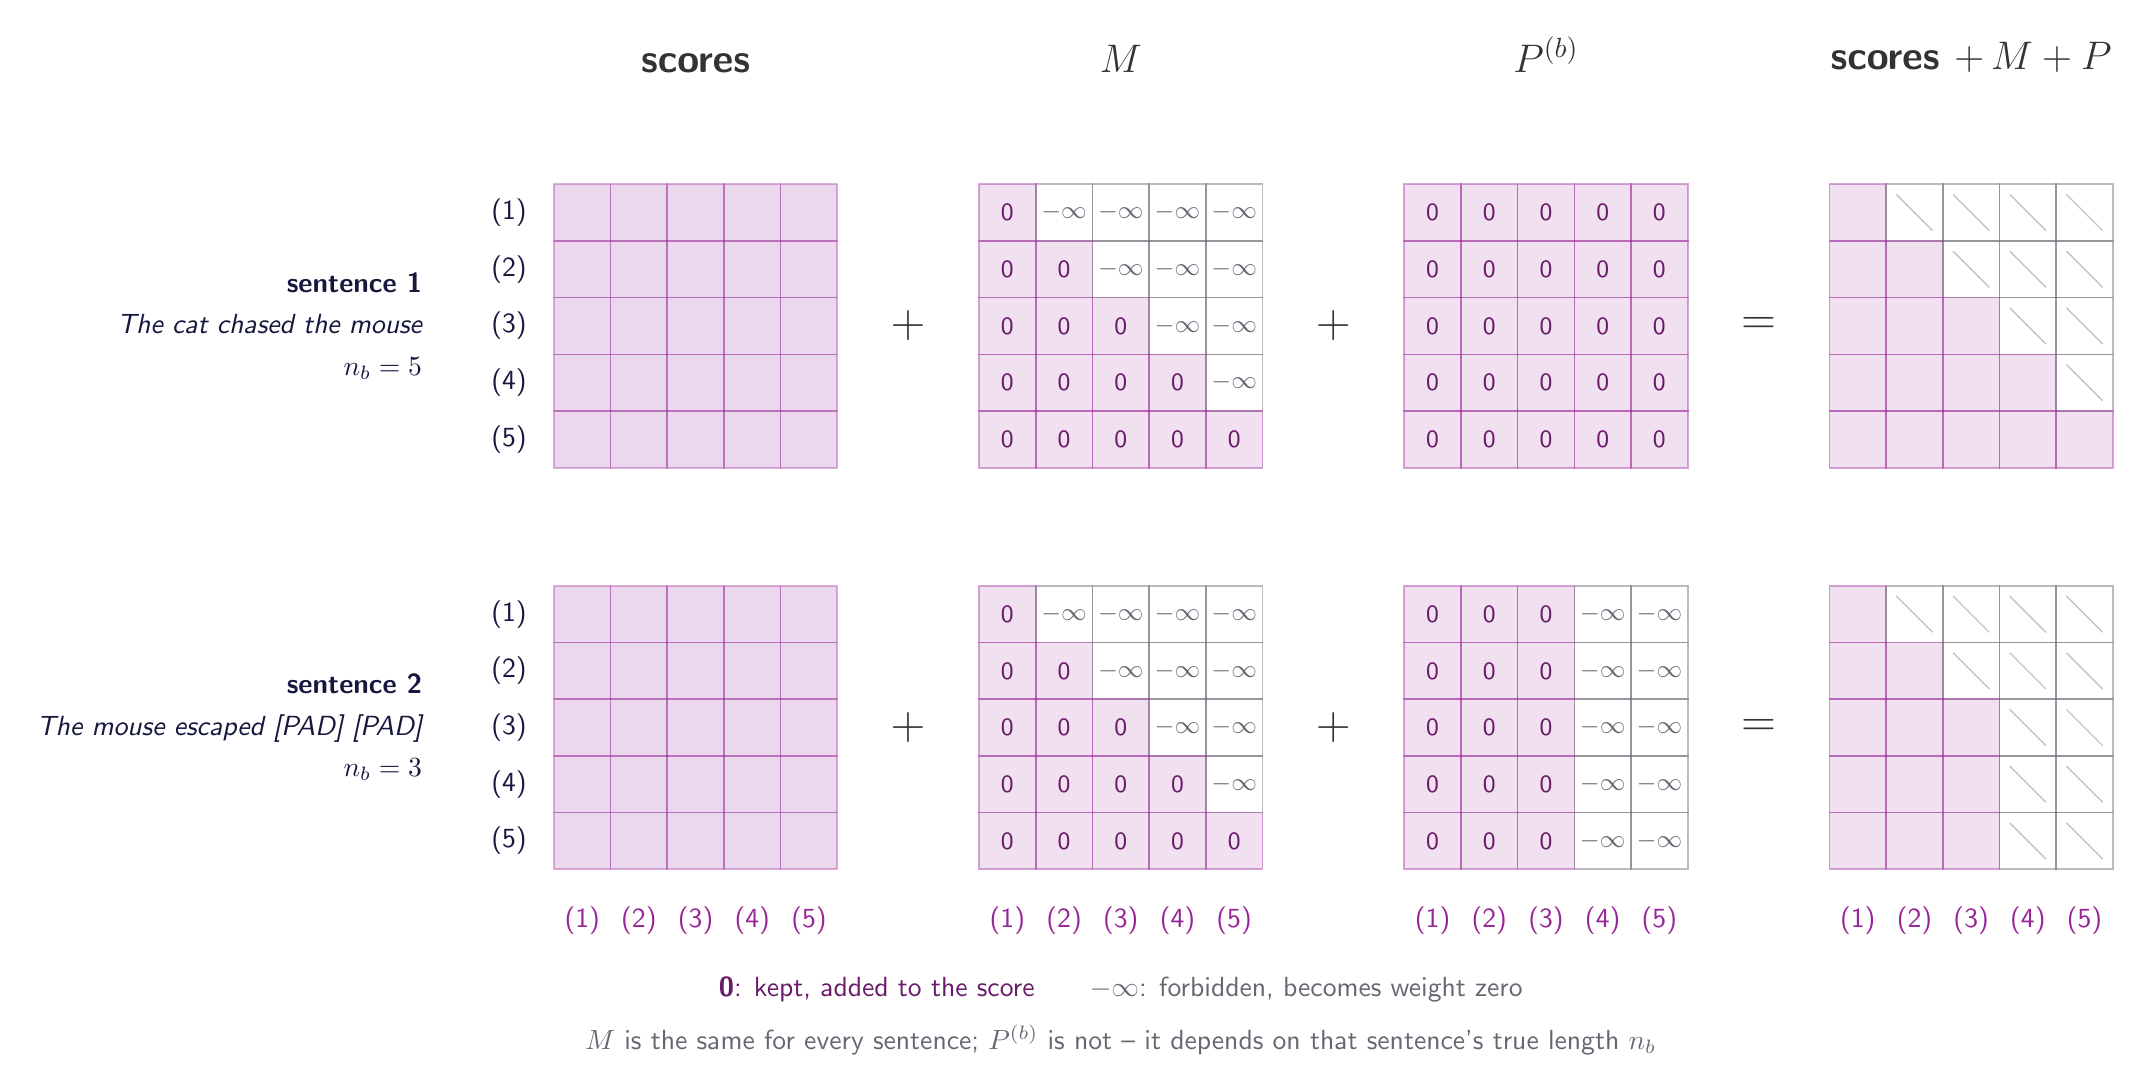
\begin{tikzpicture}[
    every node/.style={font=\sffamily},
]

% ---------------------------------------------------------------- colours
\definecolor{c1}{HTML}{15173D}   % rows, query position
\definecolor{c2}{HTML}{982598}   % kept cells, columns being read
\definecolor{c3}{HTML}{E491C9}
\definecolor{c4}{HTML}{F1E9E9}
\definecolor{axiscolor}{HTML}{333333}
\definecolor{labelcolor}{HTML}{6B6472}

% ================================================================
% Geometry, decided before any TikZ was written.
%
%   two rows, one per sentence in the batch: M is identical in both, only
%   P^(b) (and therefore the kept region) changes with the sentence
%
%   four 5x5 grids per row, cell 0.72, so each grid is 3.60 x 3.60
%   pitch between grid origins 5.40  ->  gap 1.80
%   panel origins: scores 0, M 5.40, P 10.80, masked 16.20
%
%   operator centred in each gap, at each row's grid mid-height y = -1.80:
%     "+" at 4.50, "+" at 9.90, "=" at 15.30  (offset by row y-shift)
%
%   row 1: sentence "The cat chased the mouse", n = 5, n_b = 5 (no padding)
%   row 2: sentence "The mouse escaped [PAD] [PAD]", n = 5, n_b = 3
%   (same two sentences as padding_batch.svg)
%
%   row 1 grid top at y = 0, row 2 grid top at y = -5.10
%   (grid height 3.60 + 1.50 gap for the row header and column labels:
%    tightened from the first draft, which had 2.25 of dead space here)
%
%   column titles once, above row 1, at y = 1.30
%   row header (sentence + n_b) to the left of each row's scores panel,
%       anchored east at x = -1.55, three lines
%   column labels once, below row 2, at y = -9.05
%   legend below that, at y = -9.95 and -10.55
%
%   bounding box roughly x in [-3.8, 19.6], y in [-11.1, 2.1]: wide and tall
% ================================================================

\def\cs{0.72}
\def\pM{5.40}
\def\pP{10.80}
\def\pF{16.20}
\def\rowB{-5.10}

\tikzset{
    keep/.style={fill=c2, fill opacity=0.14, draw=c2, draw opacity=0.40,
                 line width=0.6pt},
    kepttext/.style={font=\sffamily\small, text=c2!70!black},
    gone/.style={draw=labelcolor, draw opacity=0.45, line width=0.6pt},
    gonetext/.style={font=\sffamily\small, text=labelcolor},
    plain/.style={fill=c2, fill opacity=0.18, draw=c2, draw opacity=0.35,
                  line width=0.6pt},
    strike/.style={draw=labelcolor, draw opacity=0.40, line width=0.5pt},
    title/.style={font=\sffamily\Large\bfseries, text=axiscolor,
                  anchor=south},
    rowhead/.style={font=\sffamily\normalsize, text=c1, anchor=east,
                    align=right},
    rowlab/.style={font=\sffamily\normalsize, text=c1, anchor=east},
    collab/.style={font=\sffamily\normalsize, text=c2, anchor=north},
    op/.style={font=\sffamily\LARGE, text=axiscolor, anchor=center},
}

% ================================================================
% one full row of four panels: scores + M + P^(b) = masked, at vertical
% shift \y, forbidding P-columns with index > \cut (0-indexed)
% ================================================================
\newcommand{\masksrow}[2]{
  \begin{scope}[shift={(0,#1)}]

    % ---------------------------------------------------------- scores
    \foreach \i in {0,...,4} {
      \foreach \j in {0,...,4} {
        \draw[plain] (\j*\cs, -\i*\cs) rectangle ++(\cs, -\cs);
      }
    }

    % ---------------------------------------------------------- M
    \begin{scope}[shift={(\pM,0)}]
      \foreach \i in {0,...,4} {
        \foreach \j in {0,...,4} {
          \ifnum\j>\i
            \draw[gone] (\j*\cs, -\i*\cs) rectangle ++(\cs, -\cs);
            \node[gonetext] at (\j*\cs+0.5*\cs, -\i*\cs-0.5*\cs) {$-\infty$};
          \else
            \draw[keep] (\j*\cs, -\i*\cs) rectangle ++(\cs, -\cs);
            \node[kepttext] at (\j*\cs+0.5*\cs, -\i*\cs-0.5*\cs) {0};
          \fi
        }
      }
    \end{scope}

    % ---------------------------------------------------------- P^(b)
    \begin{scope}[shift={(\pP,0)}]
      \foreach \i in {0,...,4} {
        \foreach \j in {0,...,4} {
          \ifnum\j>#2
            \draw[gone] (\j*\cs, -\i*\cs) rectangle ++(\cs, -\cs);
            \node[gonetext] at (\j*\cs+0.5*\cs, -\i*\cs-0.5*\cs) {$-\infty$};
          \else
            \draw[keep] (\j*\cs, -\i*\cs) rectangle ++(\cs, -\cs);
            \node[kepttext] at (\j*\cs+0.5*\cs, -\i*\cs-0.5*\cs) {0};
          \fi
        }
      }
    \end{scope}

    % ---------------------------------------------------------- masked
    \begin{scope}[shift={(\pF,0)}]
      \foreach \i in {0,...,4} {
        \foreach \j in {0,...,4} {
          \ifnum\j>\i
            \draw[gone] (\j*\cs, -\i*\cs) rectangle ++(\cs, -\cs);
            \draw[strike] (\j*\cs+0.13, -\i*\cs-0.13) -- ++(0.46, -0.46);
          \else
            \ifnum\j>#2
              \draw[gone] (\j*\cs, -\i*\cs) rectangle ++(\cs, -\cs);
              \draw[strike] (\j*\cs+0.13, -\i*\cs-0.13) -- ++(0.46, -0.46);
            \else
              \draw[keep] (\j*\cs, -\i*\cs) rectangle ++(\cs, -\cs);
            \fi
          \fi
        }
      }
    \end{scope}

    % ---------------------------------------------------------- row labels
    \foreach \i in {0,...,4} {
      \pgfmathtruncatemacro{\p}{\i+1}
      \node[rowlab] at (-0.22, -\i*\cs-0.5*\cs) {(\p)};
    }

    % ---------------------------------------------------------- operators
    \node[op] at (4.50, -1.80) {$+$};
    \node[op] at (9.90, -1.80) {$+$};
    \node[op] at (15.30, -1.80) {$=$};
  \end{scope}
}

% ---------------------------------------------------------------- row 1
\masksrow{0}{4}
\node[rowhead] at (-1.55, -1.80)
    {\textbf{sentence 1}\\[3pt] \normalsize\itshape The cat chased the mouse
     \\[3pt] $n_b = 5$};

% ---------------------------------------------------------------- row 2
\masksrow{\rowB}{2}
\node[rowhead] at (-1.55, {\rowB-1.80})
    {\textbf{sentence 2}\\[3pt] \normalsize\itshape
     The mouse escaped [PAD] [PAD] \\[3pt] $n_b = 3$};

% ---------------------------------------------------------------- column titles
\node[title] at (1.80, 1.30) {scores};
\node[title] at (\pM+1.80, 1.30) {$M$};
\node[title] at (\pP+1.80, 1.30) {$P^{(b)}$};
\node[title] at (\pF+1.80, 1.30) {scores $+\,M+P$};

% ---------------------------------------------------------------- column labels
\foreach \px in {0, \pM, \pP, \pF} {
  \foreach \j in {0,...,4} {
    \pgfmathtruncatemacro{\p}{\j+1}
    \node[collab] at ({\px+\j*\cs+0.5*\cs}, -9.05) {(\p)};
  }
}

% ---------------------------------------------------------------- legend
\node[font=\sffamily\normalsize, anchor=north] at (\pM+1.80, -9.95)
    {\textcolor{c2!70!black}{\textbf{0}: kept, added to the score}\qquad
     \textcolor{labelcolor}{\textbf{$-\infty$}: forbidden, becomes weight zero}};
\node[font=\sffamily\normalsize, text=labelcolor, anchor=north]
    at (\pM+1.80, -10.55)
    {$M$ is the same for every sentence; $P^{(b)}$ is not --
     it depends on that sentence's true length $n_b$};

\end{tikzpicture}
\end{document}
